\clearpage
\SourceLeaf{273}%
\begin{center}
\textbf{[ÜBER DIE SUMME DER AUSSENWINKEL EINES POLYGONS.]}

\medskip
\textsc{Gauss} an \textsc{Gerling}. \quad Göttingen, 2. October 1846.
\end{center}

\mbox{.\,.\,.\,.\,.\,.} Der Satz, den Ihnen Hr. \textsc{Schweikart} erwähnt hat, dass in jeder Geometrie die Summe aller äussern Polygonwinkel von $360^0$ um eine Grösse verschieden ist (nemlich kleiner als $360^0$ in der Astralgeometrie, wie \textsc{Schw.} sie aufgefasst hat), welche dem Flächeninhalt proportional ist, ist der erste gleichsam an der Schwelle liegende Satz der Theorie, den ich schon im Jahr 1794 als nothwendig erkannte. Zu weitern Bemerkungen fehlt mir aber diessmal alle Zeit.

\begin{center}
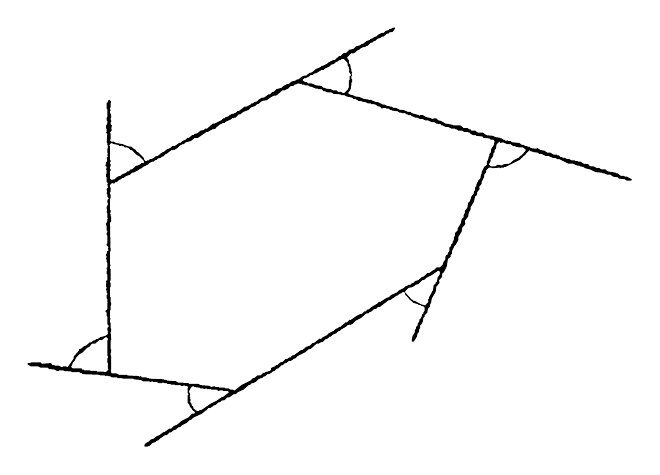
\begin{tikzpicture}[x=0.00823045cm,y=-0.00823045cm]
\fill[even odd rule] (953,265) -- (945,261) -- (942,261) -- (941,260) -- (936,260) -- (931,256) -- (929,256) -- (928,255) -- (916,253) -- (912,250) -- (906,250) -- (903,248) -- (899,248) -- (893,245) -- (889,245) -- (887,244) -- (886,242) -- (878,241) -- (874,238) -- (870,238) -- (869,237) -- (866,237) -- (865,236) -- (860,236) -- (856,234) -- (853,234) -- (849,232) -- (846,232) -- (845,231) -- (843,231) -- (840,228) -- (838,228) -- (837,227) -- (832,227) -- (827,224) -- (822,224) -- (818,221) -- (812,220) -- (807,217) -- (805,218) -- (797,217) -- (795,215) -- (792,215) -- (791,214) -- (788,214) -- (786,212) -- (783,212) -- (779,209) -- (768,208) -- (765,206) -- (762,206) -- (761,205) -- (758,206) -- (756,204) -- (754,204) -- (752,202) -- (750,202) -- (749,201) -- (742,200) -- (738,198) -- (728,197) -- (723,193) -- (715,193) -- (711,190) -- (705,190) -- (704,188) -- (702,188) -- (699,186) -- (693,186) -- (688,182) -- (677,182) -- (676,181) -- (665,179) -- (658,175) -- (654,174) -- (651,171) -- (647,171) -- (646,172) -- (644,172) -- (643,171) -- (635,169) -- (630,166) -- (627,166) -- (625,167) -- (624,166) -- (613,163) -- (611,161) -- (607,161) -- (600,158) -- (595,158) -- (589,155) -- (585,155) -- (582,153) -- (579,153) -- (578,152) -- (575,152) -- (572,150) -- (569,150) -- (561,146) -- (558,146) -- (551,143) -- (547,143) -- (546,142) -- (539,141) -- (532,138) -- (525,137) -- (524,136) -- (517,134) -- (515,132) -- (515,131) -- (517,129) -- (519,125) -- (519,121) -- (520,120) -- (520,116) -- (521,115) -- (521,111) -- (520,110) -- (520,106) -- (521,105) -- (520,102) -- (521,100) -- (520,99) -- (520,95) -- (519,94) -- (518,88) -- (516,86) -- (516,82) -- (513,77) -- (519,71) -- (521,70) -- (522,71) -- (526,69) -- (529,66) -- (532,65) -- (534,63) -- (538,61) -- (541,61) -- (543,59) -- (545,59) -- (550,54) -- (552,54) -- (554,52) -- (557,51) -- (560,48) -- (564,47) -- (567,45) -- (569,45) -- (575,40) -- (577,40) -- (579,38) -- (583,38) -- (587,33) -- (587,31) -- (584,31) -- (581,33) -- (579,33) -- (577,35) -- (573,36) -- (570,39) -- (567,39) -- (561,42) -- (558,45) -- (556,45) -- (552,48) -- (550,48) -- (548,50) -- (543,52) -- (538,56) -- (536,56) -- (534,58) -- (527,60) -- (523,64) -- (517,65) -- (512,70) -- (509,70) -- (507,71) -- (503,75) -- (501,75) -- (494,81) -- (492,81) -- (484,85) -- (482,87) -- (476,90) -- (474,90) -- (472,92) -- (465,95) -- (459,100) -- (455,101) -- (450,105) -- (447,105) -- (443,107) -- (438,111) -- (436,111) -- (433,113) -- (428,114) -- (423,118) -- (421,118) -- (415,121) -- (412,124) -- (404,126) -- (400,130) -- (398,130) -- (394,134) -- (392,134) -- (385,139) -- (382,139) -- (377,142) -- (374,145) -- (370,146) -- (368,148) -- (366,148) -- (364,150) -- (358,153) -- (355,153) -- (346,160) -- (344,160) -- (342,162) -- (338,164) -- (336,164) -- (332,166) -- (330,168) -- (326,169) -- (324,171) -- (322,171) -- (319,174) -- (309,179) -- (306,179) -- (297,187) -- (294,187) -- (292,189) -- (287,190) -- (282,194) -- (278,195) -- (276,197) -- (274,197) -- (269,201) -- (267,201) -- (264,204) -- (259,206) -- (256,209) -- (254,209) -- (247,214) -- (243,214) -- (240,217) -- (235,219) -- (230,223) -- (227,224) -- (221,229) -- (217,230) -- (215,232) -- (211,234) -- (209,234) -- (207,236) -- (205,236) -- (204,237) -- (202,237) -- (200,235) -- (199,232) -- (190,223) -- (189,223) -- (186,219) -- (185,219) -- (180,215) -- (174,214) -- (167,211) -- (156,209) -- (153,207) -- (149,207) -- (147,205) -- (148,203) -- (148,195) -- (147,193) -- (150,189) -- (149,187) -- (150,182) -- (148,180) -- (148,177) -- (149,176) -- (149,174) -- (148,173) -- (148,171) -- (149,170) -- (149,166) -- (147,162) -- (147,160) -- (148,159) -- (147,155) -- (148,154) -- (148,147) -- (149,146) -- (147,143) -- (145,143) -- (144,144) -- (144,146) -- (142,147) -- (142,156) -- (143,157) -- (143,169) -- (142,170) -- (142,174) -- (143,175) -- (143,179) -- (141,183) -- (141,186) -- (142,187) -- (142,192) -- (141,193) -- (143,195) -- (142,208) -- (143,209) -- (143,212) -- (144,213) -- (144,217) -- (143,218) -- (143,224) -- (144,225) -- (143,228) -- (144,230) -- (142,232) -- (143,237) -- (141,239) -- (141,242) -- (140,243) -- (140,244) -- (142,246) -- (142,248) -- (141,249) -- (142,251) -- (142,256) -- (141,257) -- (141,261) -- (142,262) -- (142,269) -- (144,271) -- (143,273) -- (144,278) -- (142,280) -- (142,282) -- (143,283) -- (142,287) -- (143,288) -- (143,292) -- (145,294) -- (145,295) -- (143,297) -- (143,301) -- (144,302) -- (144,304) -- (142,308) -- (142,311) -- (143,312) -- (142,316) -- (143,317) -- (143,324) -- (144,326) -- (143,327) -- (143,330) -- (141,334) -- (141,336) -- (142,337) -- (142,344) -- (143,345) -- (143,347) -- (142,348) -- (142,351) -- (143,352) -- (143,364) -- (142,365) -- (142,367) -- (145,370) -- (144,372) -- (145,375) -- (143,376) -- (142,380) -- (141,381) -- (141,383) -- (142,384) -- (141,388) -- (142,389) -- (142,393) -- (143,394) -- (143,401) -- (142,402) -- (142,404) -- (143,405) -- (142,407) -- (142,411) -- (143,412) -- (143,421) -- (141,422) -- (141,424) -- (142,425) -- (141,427) -- (141,431) -- (142,432) -- (141,436) -- (142,437) -- (142,440) -- (143,441) -- (143,443) -- (142,444) -- (142,449) -- (143,450) -- (143,454) -- (144,455) -- (143,456) -- (143,466) -- (141,468) -- (140,468) -- (140,469) -- (142,471) -- (142,476) -- (143,477) -- (143,489) -- (145,491) -- (145,493) -- (143,495) -- (143,498) -- (144,499) -- (144,504) -- (140,507) -- (132,509) -- (128,512) -- (126,512) -- (124,514) -- (122,514) -- (118,517) -- (116,517) -- (110,522) -- (107,523) -- (102,527) -- (100,527) -- (99,528) -- (99,530) -- (91,539) -- (91,542) -- (82,555) -- (80,555) -- (79,554) -- (75,554) -- (74,555) -- (72,555) -- (68,553) -- (62,553) -- (61,552) -- (58,552) -- (57,550) -- (55,549) -- (42,550) -- (40,548) -- (25,548) -- (24,549) -- (20,549) -- (20,551) -- (25,554) -- (36,554) -- (40,556) -- (51,556) -- (53,558) -- (62,559) -- (65,561) -- (68,561) -- (69,560) -- (75,560) -- (76,561) -- (88,562) -- (89,563) -- (100,563) -- (101,564) -- (103,564) -- (105,566) -- (131,567) -- (132,568) -- (139,568) -- (140,569) -- (143,568) -- (144,569) -- (147,569) -- (150,571) -- (158,571) -- (159,572) -- (166,572) -- (167,573) -- (183,573) -- (184,574) -- (195,575) -- (198,577) -- (208,577) -- (209,578) -- (213,577) -- (214,578) -- (219,578) -- (223,580) -- (227,580) -- (228,579) -- (230,579) -- (231,580) -- (235,580) -- (236,581) -- (240,581) -- (241,582) -- (247,582) -- (248,583) -- (256,583) -- (257,584) -- (260,584) -- (262,583) -- (263,584) -- (266,584) -- (268,586) -- (267,588) -- (267,595) -- (268,596) -- (268,598) -- (267,599) -- (267,610) -- (269,612) -- (271,617) -- (274,620) -- (274,621) -- (278,624) -- (278,626) -- (277,627) -- (274,627) -- (268,633) -- (258,638) -- (251,644) -- (246,646) -- (242,650) -- (239,650) -- (232,655) -- (229,656) -- (224,660) -- (219,662) -- (214,666) -- (210,667) -- (207,670) -- (202,673) -- (200,676) -- (201,678) -- (205,678) -- (206,677) -- (208,677) -- (213,672) -- (217,671) -- (219,669) -- (222,668) -- (226,664) -- (227,664) -- (232,660) -- (235,660) -- (239,656) -- (241,656) -- (246,652) -- (248,652) -- (253,648) -- (255,648) -- (258,645) -- (266,641) -- (270,637) -- (273,636) -- (276,633) -- (289,627) -- (295,622) -- (296,622) -- (299,618) -- (302,618) -- (304,617) -- (306,615) -- (311,613) -- (314,610) -- (317,609) -- (319,607) -- (324,606) -- (328,602) -- (331,602) -- (338,597) -- (341,597) -- (344,594) -- (353,590) -- (361,583) -- (364,582) -- (366,580) -- (368,580) -- (372,578) -- (376,574) -- (380,572) -- (382,572) -- (384,570) -- (387,569) -- (390,566) -- (392,566) -- (396,564) -- (398,562) -- (401,561) -- (404,558) -- (407,557) -- (412,552) -- (414,552) -- (417,549) -- (419,549) -- (424,545) -- (425,546) -- (429,544) -- (431,542) -- (433,542) -- (437,538) -- (449,532) -- (453,528) -- (457,527) -- (466,519) -- (469,519) -- (472,517) -- (476,516) -- (480,512) -- (483,511) -- (486,508) -- (488,508) -- (491,505) -- (496,503) -- (499,500) -- (502,499) -- (504,497) -- (511,493) -- (514,490) -- (516,490) -- (517,489) -- (518,490) -- (522,488) -- (527,483) -- (535,479) -- (543,472) -- (546,472) -- (548,470) -- (551,469) -- (554,466) -- (558,465) -- (561,462) -- (564,462) -- (577,452) -- (581,451) -- (583,449) -- (584,449) -- (589,445) -- (592,444) -- (594,442) -- (597,441) -- (599,439) -- (601,439) -- (603,441) -- (603,443) -- (607,447) -- (607,448) -- (608,448) -- (609,450) -- (616,456) -- (623,458) -- (624,459) -- (626,459) -- (629,461) -- (631,461) -- (633,463) -- (633,468) -- (631,471) -- (631,473) -- (629,474) -- (629,476) -- (627,480) -- (625,482) -- (625,484) -- (622,489) -- (622,491) -- (620,493) -- (620,495) -- (618,498) -- (618,501) -- (614,508) -- (613,515) -- (615,516) -- (618,513) -- (621,508) -- (622,503) -- (624,501) -- (624,498) -- (626,494) -- (626,491) -- (628,489) -- (630,485) -- (631,479) -- (633,477) -- (633,475) -- (637,471) -- (638,465) -- (641,462) -- (641,459) -- (643,455) -- (644,449) -- (650,439) -- (651,431) -- (656,425) -- (655,421) -- (659,417) -- (660,415) -- (660,411) -- (663,408) -- (667,400) -- (669,388) -- (673,385) -- (673,382) -- (675,380) -- (675,376) -- (679,368) -- (681,366) -- (685,359) -- (685,354) -- (690,346) -- (691,340) -- (696,334) -- (695,332) -- (695,329) -- (700,323) -- (701,317) -- (704,311) -- (704,308) -- (709,300) -- (711,291) -- (713,290) -- (714,288) -- (714,285) -- (718,280) -- (717,277) -- (721,272) -- (721,269) -- (725,261) -- (725,258) -- (728,254) -- (728,251) -- (732,247) -- (736,247) -- (737,248) -- (749,247) -- (750,248) -- (751,247) -- (755,247) -- (756,246) -- (758,246) -- (780,235) -- (787,228) -- (788,228) -- (789,226) -- (795,220) -- (797,222) -- (799,222) -- (800,223) -- (808,224) -- (810,226) -- (814,226) -- (820,229) -- (824,229) -- (831,232) -- (835,232) -- (838,234) -- (841,234) -- (855,241) -- (862,241) -- (869,244) -- (872,244) -- (873,245) -- (878,246) -- (881,248) -- (889,250) -- (897,254) -- (907,255) -- (908,256) -- (911,256) -- (915,258) -- (920,258) -- (924,261) -- (931,262) -- (933,264) -- (942,265) -- (945,267) -- (952,267) -- cycle
(269,593) -- (272,587) -- (274,585) -- (277,585) -- (278,586) -- (286,587) -- (287,588) -- (291,588) -- (292,589) -- (296,588) -- (297,589) -- (303,589) -- (304,590) -- (312,590) -- (315,592) -- (317,591) -- (321,591) -- (322,592) -- (329,592) -- (331,594) -- (322,601) -- (319,602) -- (312,607) -- (302,612) -- (289,621) -- (285,622) -- (284,623) -- (281,623) -- (276,619) -- (276,617) -- (273,614) -- (273,612) -- (271,609) -- (271,607) -- (272,606) -- (271,605) -- (271,602) -- (270,601) -- (271,597) -- cycle
(144,511) -- (144,513) -- (143,514) -- (143,537) -- (144,538) -- (144,541) -- (143,542) -- (143,548) -- (144,549) -- (144,557) -- (145,559) -- (141,563) -- (138,563) -- (137,562) -- (127,562) -- (126,561) -- (117,561) -- (116,560) -- (107,560) -- (106,559) -- (104,559) -- (103,557) -- (89,557) -- (87,555) -- (90,548) -- (92,546) -- (95,540) -- (100,535) -- (104,533) -- (112,525) -- (115,524) -- (119,519) -- (124,519) -- (131,513) -- (135,513) -- (140,509) -- (142,509) -- cycle
(656,407) -- (657,410) -- (656,411) -- (656,413) -- (653,417) -- (652,423) -- (650,425) -- (650,426) -- (648,428) -- (647,428) -- (646,436) -- (640,447) -- (640,449) -- (638,451) -- (639,454) -- (634,460) -- (627,458) -- (618,453) -- (616,453) -- (614,451) -- (613,451) -- (603,440) -- (603,438) -- (609,432) -- (610,433) -- (611,432) -- (613,432) -- (617,430) -- (619,428) -- (623,427) -- (629,421) -- (633,420) -- (636,417) -- (644,413) -- (654,406) -- cycle
(147,211) -- (149,209) -- (154,211) -- (160,212) -- (162,214) -- (165,213) -- (166,214) -- (168,214) -- (170,216) -- (174,216) -- (176,217) -- (179,220) -- (181,220) -- (189,228) -- (192,229) -- (199,236) -- (200,239) -- (199,240) -- (196,240) -- (194,242) -- (190,244) -- (188,244) -- (181,250) -- (179,250) -- (176,253) -- (174,253) -- (172,255) -- (165,258) -- (163,260) -- (159,261) -- (153,266) -- (152,265) -- (151,266) -- (149,266) -- (147,264) -- (147,253) -- (148,252) -- (148,250) -- (147,249) -- (147,246) -- (148,245) -- (148,242) -- (147,241) -- (147,239) -- (148,238) -- (148,236) -- (147,235) -- (147,214) -- (146,213) -- cycle
(732,242) -- (735,237) -- (735,234) -- (737,232) -- (739,228) -- (739,225) -- (741,223) -- (741,220) -- (743,218) -- (744,211) -- (748,207) -- (749,207) -- (750,209) -- (754,208) -- (761,211) -- (766,211) -- (770,214) -- (773,214) -- (774,215) -- (777,215) -- (778,216) -- (785,216) -- (789,219) -- (789,221) -- (783,228) -- (782,228) -- (778,232) -- (770,236) -- (764,241) -- (755,242) -- (751,244) -- (749,243) -- (745,243) -- (742,245) -- (735,245) -- cycle
(741,206) -- (740,212) -- (736,218) -- (735,224) -- (733,226) -- (733,229) -- (732,230) -- (731,235) -- (729,238) -- (729,243) -- (725,246) -- (721,254) -- (721,257) -- (720,258) -- (719,264) -- (716,267) -- (713,273) -- (713,275) -- (711,278) -- (711,282) -- (709,284) -- (709,287) -- (705,292) -- (703,299) -- (700,302) -- (699,309) -- (695,314) -- (695,317) -- (693,321) -- (693,324) -- (690,327) -- (689,333) -- (684,341) -- (684,344) -- (680,348) -- (680,352) -- (678,355) -- (678,359) -- (676,362) -- (676,364) -- (674,366) -- (674,368) -- (671,371) -- (671,376) -- (669,379) -- (669,381) -- (667,382) -- (665,385) -- (665,389) -- (662,393) -- (661,397) -- (657,401) -- (652,401) -- (648,405) -- (647,405) -- (640,410) -- (637,410) -- (632,415) -- (629,416) -- (623,421) -- (619,422) -- (616,425) -- (613,426) -- (611,428) -- (608,428) -- (606,430) -- (604,430) -- (601,433) -- (593,437) -- (590,440) -- (581,444) -- (578,447) -- (573,449) -- (564,455) -- (563,454) -- (560,457) -- (550,463) -- (547,466) -- (545,466) -- (542,469) -- (540,469) -- (536,473) -- (534,473) -- (528,476) -- (518,483) -- (517,482) -- (513,486) -- (511,486) -- (503,493) -- (501,493) -- (499,495) -- (496,496) -- (493,499) -- (485,503) -- (482,506) -- (476,509) -- (473,512) -- (471,511) -- (462,518) -- (460,518) -- (456,522) -- (450,524) -- (444,529) -- (442,529) -- (431,537) -- (429,537) -- (425,541) -- (424,540) -- (422,542) -- (418,543) -- (414,547) -- (410,548) -- (406,552) -- (404,552) -- (402,554) -- (397,556) -- (396,557) -- (396,559) -- (394,561) -- (387,563) -- (386,564) -- (384,564) -- (380,568) -- (375,568) -- (370,572) -- (368,572) -- (364,576) -- (350,583) -- (340,591) -- (338,591) -- (337,590) -- (333,590) -- (330,588) -- (325,588) -- (324,587) -- (316,587) -- (315,586) -- (310,586) -- (309,585) -- (306,585) -- (304,586) -- (300,584) -- (287,583) -- (283,581) -- (269,581) -- (268,580) -- (261,580) -- (260,579) -- (252,579) -- (249,577) -- (235,576) -- (234,575) -- (231,575) -- (230,574) -- (208,573) -- (207,572) -- (204,572) -- (203,571) -- (196,571) -- (195,569) -- (192,570) -- (191,569) -- (174,568) -- (173,567) -- (161,567) -- (157,565) -- (150,565) -- (149,564) -- (149,562) -- (148,561) -- (149,559) -- (149,538) -- (148,537) -- (148,533) -- (149,532) -- (149,528) -- (148,527) -- (148,514) -- (149,513) -- (148,501) -- (149,500) -- (149,496) -- (148,495) -- (148,487) -- (147,486) -- (147,482) -- (148,481) -- (147,479) -- (147,468) -- (148,467) -- (148,460) -- (149,459) -- (149,456) -- (148,455) -- (148,447) -- (147,446) -- (147,432) -- (148,431) -- (148,425) -- (147,424) -- (147,422) -- (148,421) -- (148,404) -- (147,403) -- (147,399) -- (148,398) -- (147,396) -- (147,377) -- (148,376) -- (147,332) -- (149,330) -- (149,323) -- (148,322) -- (148,319) -- (147,318) -- (148,316) -- (148,313) -- (147,312) -- (147,295) -- (148,294) -- (148,289) -- (147,288) -- (147,285) -- (148,284) -- (148,278) -- (147,277) -- (147,274) -- (150,271) -- (152,271) -- (153,272) -- (156,269) -- (158,269) -- (161,266) -- (164,265) -- (166,263) -- (168,263) -- (172,260) -- (178,258) -- (181,255) -- (183,255) -- (191,251) -- (193,249) -- (196,248) -- (198,246) -- (206,242) -- (208,240) -- (212,238) -- (214,238) -- (216,236) -- (219,235) -- (221,233) -- (225,232) -- (227,230) -- (229,230) -- (233,226) -- (234,226) -- (242,220) -- (244,220) -- (245,219) -- (246,220) -- (251,217) -- (255,213) -- (259,211) -- (261,211) -- (264,208) -- (272,206) -- (278,201) -- (283,201) -- (296,192) -- (298,192) -- (305,188) -- (310,187) -- (311,185) -- (316,181) -- (322,178) -- (324,178) -- (326,176) -- (333,173) -- (337,170) -- (338,171) -- (339,170) -- (341,170) -- (346,165) -- (348,165) -- (353,161) -- (361,158) -- (365,154) -- (371,152) -- (374,149) -- (376,149) -- (382,144) -- (389,143) -- (396,138) -- (400,136) -- (403,136) -- (405,135) -- (413,128) -- (416,128) -- (422,125) -- (425,122) -- (427,121) -- (430,121) -- (432,119) -- (436,118) -- (437,117) -- (443,118) -- (444,119) -- (447,119) -- (448,120) -- (453,120) -- (456,122) -- (458,122) -- (465,125) -- (468,125) -- (469,126) -- (474,126) -- (477,129) -- (479,129) -- (483,131) -- (489,131) -- (492,133) -- (503,134) -- (504,135) -- (509,135) -- (512,137) -- (521,139) -- (523,141) -- (526,141) -- (531,144) -- (535,144) -- (536,145) -- (542,146) -- (546,148) -- (550,148) -- (551,149) -- (555,149) -- (556,150) -- (558,150) -- (560,152) -- (564,153) -- (567,156) -- (569,155) -- (573,155) -- (574,156) -- (578,156) -- (580,158) -- (582,158) -- (583,159) -- (591,160) -- (594,162) -- (597,162) -- (598,163) -- (603,163) -- (605,165) -- (607,165) -- (608,166) -- (612,166) -- (613,168) -- (615,168) -- (619,170) -- (622,170) -- (626,172) -- (630,172) -- (634,174) -- (638,174) -- (644,177) -- (648,177) -- (651,179) -- (658,180) -- (659,182) -- (661,182) -- (665,184) -- (669,184) -- (675,187) -- (680,187) -- (681,188) -- (683,188) -- (685,190) -- (691,190) -- (694,192) -- (700,192) -- (701,193) -- (703,193) -- (704,195) -- (708,197) -- (712,197) -- (713,198) -- (722,199) -- (724,201) -- (733,202) -- (735,204) -- (739,204) -- cycle
(519,103) -- (519,105) -- (517,106) -- (517,112) -- (516,113) -- (516,123) -- (514,127) -- (509,132) -- (507,132) -- (503,130) -- (499,130) -- (497,128) -- (492,128) -- (488,126) -- (480,125) -- (479,124) -- (477,124) -- (474,121) -- (465,120) -- (458,117) -- (453,117) -- (451,115) -- (448,115) -- (444,112) -- (447,109) -- (449,109) -- (455,106) -- (457,104) -- (460,104) -- (462,102) -- (466,101) -- (474,96) -- (477,96) -- (479,94) -- (486,91) -- (489,88) -- (493,87) -- (496,84) -- (499,83) -- (501,81) -- (503,81) -- (505,79) -- (508,79) -- (513,84) -- (514,86) -- (514,89) -- (516,92) -- (516,95) -- (517,96) -- (516,99) -- cycle;
\end{tikzpicture}

\end{center}

\Needspace{6\baselineskip}
\begin{center}\textsc{Bemerkung.}\end{center}

In \textsc{Schweikarts} Astralgeometrie ist die Summe aller äussern Polygonwinkel nicht kleiner, sondern grösser als $360^0$.

\hfill \textsc{Stäckel}.
